
性能是設計目標之一,與其他需求同等重要。因此,“這種設計導致了糟糕的性能”問題的回答與“這種設計沒有提供我們需要的功能”問題的答案是一樣的。兩種情況下,都需要不同的設計。只是更習慣於根據他們做的怎麼樣來評估設計,而不是做得有多快。

為了在第一次嘗試時,選擇性能提升設計實踐,現在介紹幾個專門針對良好性能的設計指南。它們也是可靠的設計原則,有理由去了解它們,遵循這些原則不會讓設計變得更糟。 

前兩條指導原則處理設計中不同組件(函數、類、模塊、過程、任何組件)的交互。首先,建議交互傳遞儘可能少的信息,以便整個系統能正常工作。其次,建議不同的組件提供儘可能多的關於交互預期結果的信息。如果認為這是一組矛盾,也沒什麼問題。設計通常是解決矛盾的藝術,兩個矛盾的陳述都正確,只是時間或空間不同。下面的例子很好地說明瞭這種(更普遍的)管理設計矛盾的方法。

\subsubsubsection{12.3.1\hspace{0.2cm}最小信息原則}

從第一條準則開始。儘可能少地交互信息,上下文在這裡非常重要,建議組件儘可能少地暴露它如何處理特定請求的信息。組件之間的交互是由約定控制的。當討論類和函數的接口時,已經習慣了這個想法,但它是一個更廣泛的概念,用比如於兩個進程之間通信的協議,這就是一個約定。 

在此類接口或交互中,作出和履行承諾的一方不應提供額外的信息。看一些具體的例子,將從實現基本隊列的類開始,然後問自己。從效率的角度來看,什麼是好的接口?

其中有一個方法允許檢查隊列是否為空。注意,調用者並沒有詢問隊列有多少元素,而只是詢問隊列是否為空。雖然隊列的某些實現可能會緩存大小,並將其與0進行比較以應對此請求。但對於其他實現,確定隊列是否為空可能比計算元素更有效。約定中,“如果隊列為空,將返回true。”即使知道大小,也不要做承諾:\textit{不要主動提供額外的信息}。這樣,後面就可以自由地更改實現了。 

類似地,入隊和出隊的方法應該只保證向隊列中添加或刪除新元素。從隊列中彈出一個元素,必須處理空隊列的情況,或者聲明未定義嘗試的結果(STL選擇的方法)。可能注意到,STL隊列從效率的角度展示了一個出色的接口,其完成了對隊列數據結構的約定,而沒有透露任何不必要的細節。特別是,\texttt{std::queue}是一種適配器,可以在幾個容器中的一個上實現。隊列可以實現為\texttt{vector}、\texttt{deque}或\texttt{list},這個例子告訴我們,接口需要隱藏實現細節。

對於接口洩漏太多實現信息的反面例子,考慮另一個STL容器,無序\texttt{set}(或\texttt{map})。\texttt{std::unor\break dered\_set}容器有一個接口,允許插入新元素並檢查給定的值是否已經在集合中(目前為止,一切正常)。根據定義,它缺乏元素的內部順序,並且標準提供的性能保證清楚地表明數據結構使用了哈希。所以,接口中顯式地引用哈希的部分是必要的,所以必須指定一個用戶給定的哈希函數。但是這個接口走遠了,通過像\texttt{bucket\_count()}這樣的方法,暴露了底層實現必須是一個帶有桶的離散鏈接哈希表,以解決哈希衝突。因此,不可能使用開放尋址哈希表創建一個完全符合STL的無序\texttt{set}。此接口限制了實現,並可能阻礙使用更高效的實現。

雖然在簡單的例子中使用了類設計,但同樣的原則也可以應用於更大模塊的API,客戶端-服務器協議,以及系統組件之間的其他交互。在設計響應請求或提供服務的組件時,只需提供簡潔的約定,並只顯示請求者所需的信息即可。

最小信息或最小承諾的設計準則,本質上是對類接口設計準則的概括:\textit{接口不應暴露實現}。此外,要考慮到糾正違反這條指導原則的行為會相當困難。若設計洩露了實現細節,那麼客戶將依賴於它們,並且若更改了實現,就會破壞客戶的代碼。因此,為性能而設計與一般的設計實踐一樣。在下一個指導方針中,我們將開始介紹不同設計目標和相應最佳實踐之間的關係。

\subsubsubsection{12.3.2\hspace{0.2cm}最大信息原則}

雖然完成請求的組件應該避免暴露可能限制實現的信息,但對於發出請求的組件來說,情況正好相反。請求者或調用者應該能夠提供關於具體需要什麼的特定信息。當然,調用方只有在有合適的接口時才提供信息,因此接口應該允許這樣的“完整”請求。

特別是,要提供最佳性能,瞭解請求背後的意圖通常很重要。同樣,通過一個例子,應該會更容易理解這個概念。
 
讓我們從一個隨機訪問序列容器開始。隨機訪問可以訪問容器中的任意第\texttt{i}個元素,而不需要訪問其他元素。通常的方法是使用索引運算符:

\begin{lstlisting}[style=styleCXX]
T& operator[](size_t i) { return … i-th element …; }
\end{lstlisting}

有了這個操作符,就可以遍歷容器了:

\begin{lstlisting}[style=styleCXX]
container<T> cont;
… add some data to cont …
for (size_t i = 0; i != cont.size(); ++i) {
	T& element_i = cont[i];
	… do some work on the i-th element …
}
\end{lstlisting}

從效率的角度來看,這不是最好的方法,因為現在使用隨機訪問迭代器進行順序迭代。對於更強大或功能更強大的接口,在只使用了它的一小部分功能時,就應該關注效率。該接口的靈活性可能會以性能為代價,如果不使用這些特性,就會浪費性能。 

假設\texttt{std::deque}是一個支持隨機訪問的塊分配容器。為了訪問任意元素\texttt{i},必須首先計算哪個塊包含這個元素(通常是一個取模操作)和塊中元素的索引,然後在輔助數據結構(塊指針表)中找到塊的地址,並在塊中進行索引。對於下一個元素,必須重複這個過程。不過在大多數情況下,元素將駐留在同一個塊中,而且我們對地址已知。這是因為對任意元素的請求沒有包含足夠的信息,沒有辦法知道將很快請求下一個元素。因此,\texttt{deque}不能以最有效的方式處理遍歷。

另一種遍歷整個容器的方法是使用迭代器:

\begin{lstlisting}[style=styleCXX]
for (auto it = cont.begin(); it != cont.end(); ++it) {
	T& element = *it;
	… do some work on the element …
}
\end{lstlisting}

\texttt{deque}的實現者可以假設迭代器的自增(或自減)操作。因此,如果有一個迭代器\texttt{it}並訪問相應的元素\texttt{*it},很可能會請求下一個元素。\texttt{deque}迭代器可以在塊指針表中存儲塊指針或右變元素的索引,這將使訪問一個塊中元素的成本更低。通過一個簡單的基準測試,可以驗證使用迭代器遍歷\texttt{deque}容器確實比索引更快:

\hspace*{\fill} \\ %插入空行
\noindent
\textbf{01\_deque.C}
\begin{lstlisting}[style=styleCXX]
void BM_index(benchmark::State& state) {
	const unsigned int N = state.range(0);
	std::deque<unsigned long> d(N);
	for (auto _ : state) {
		for (size_t i = 0; i < N; ++i) {
			benchmark::DoNotOptimize(d[i]);
		}
		benchmark::ClobberMemory();
	}
	state.SetItemsProcessed(N*state.iterations());
}
void BM_iter(benchmark::State& state) {
	const unsigned int N = state.range(0);
	std::deque<unsigned long> d(N);
	for (auto _ : state) {
		for (auto it = d.cbegin(), it0 = d.cend(); 
		it != it0; ++it) {
			benchmark::DoNotOptimize(*it);
		}
		benchmark::ClobberMemory();
	}
	state.SetItemsProcessed(N*state.iterations());
}
\end{lstlisting}

性能差異顯著:

\hspace*{\fill} \\ %插入空行
\begin{center}
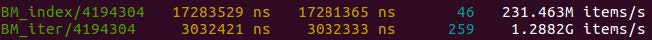
\includegraphics[width=0.9\textwidth]{content/3/chapter12/images/1.jpg}\\
圖12.1 - 使用索引和迭代器遍歷\texttt{std::deque}
\end{center}

指出為性能而設計和為性能而優化之間的關鍵區別非常重要。不能保證迭代器訪問\texttt{deque}容器的速度更快,特定的實現可能會使用索引操作符來實現迭代器,這樣的保證可能來自一個優化的實現。本章中,我們感興趣的是設計。儘管,談論“有效的設計”時,其他人可能會理解這話的意思,但設計不能真正地“優化”。設計可以允許或阻止某些優化,所以更準確的說法是“性能敵對”或“性能友好”的設計(後者通常也稱為有效設計)。

在\texttt{deque}示例中,索引操作符對於隨機訪問是高效的,並且將順序迭代視為隨機訪問的一種特殊情況。調用者不可能說:“接下來我可能會請求相鄰的元素。”相反,根據迭代器的存在性,可以推斷它可能是遞增或遞減的。該實現可以使這種增量操作執行的更高效。

進一步討論容器的例子。這一次,考慮一個自定義容器,功能上是一個樹,但與\texttt{std::set}不同,不將值存儲在樹節點中。相反,將值存儲在序列容器(數據存儲)中,而樹節點包含指向該容器元素的指針。樹本質上是數據存儲的索引,因此需要一個定製的比較函數。這裡想要比較的是值,而不是指針。

\hspace*{\fill} \\ %插入空行
\noindent
\textbf{02\_index\_tree.C}
\begin{lstlisting}[style=styleCXX]
template<typename T> struct compare_ptr {
	bool operator()(const T* a, const T* b) const {
		return *a < *b;
	}
};
template <typename T> class index_tree {
	public:
	void insert(const T& t) { 
		data_.push_back(t);
		idx_.insert(&(data_[data_.size() - 1]));
	}
	private:
	std::set<T*, compare_ptr<T>> idx_;
	std::vector<T> data_;
};
\end{lstlisting}

插入新元素時,將添加到數據存儲的末尾,而指針將添加到由元素比較確定的索引位置。為什麼要選擇這樣的實現,而不是\texttt{std::set}呢?某些情況下,可能會有強制的需求,例如:數據存儲可能是磁盤上的內存映射文件。其他情況下,為了提高性能,可以選擇這種實現。可能乍一看,額外的內存使用和通過指針間接訪問元素會降低性能。 

為了瞭解這個索引樹容器的性能優勢,檢查搜索滿足給定謂詞的元素的操作。假設容器提供了迭代器,可以簡單地遍歷索引集,就可以輕鬆地進行搜索。解引用操作符應該返回索引的元素值,而不是指針:

\hspace*{\fill} \\ %插入空行
\noindent
\textbf{02\_index\_tree.C}
\begin{lstlisting}[style=styleCXX]
template <typename T> class index_tree {
	using idx_t = typename std::set<T*, compare_ptr<T>>;
	using idx_iter_t = typename idx_t::const_iterator;
	public:
	class const_iterator {
		idx_iter_t it_;
		public:
		const_iterator(idx_iter_t it) : it_(it) {}
		const_iterator operator++() { ++it_; return *this; }
		const T& operator*() const { return *(*it_); }
		friend bool operator!=(const const_iterator& a,
		const const_iterator& b) {
			return a.it_ != b.it_;
		}
	};
	const_iterator cbegin() const { return idx_.cbegin(); }
	const_iterator cend() const { return idx_.cend(); }
	…
};
\end{lstlisting}

要確定一個滿足特定要求的值是否已經存儲在容器中,只需遍歷整個容器,並檢查每個值的謂詞:

\begin{lstlisting}[style=styleCXX]
template <typename C, typename F> bool find(const C& c, F f) {
	for (auto it = c.cbegin(), i0 = c.cend(); it != i0; ++it) {
		if (f(*it)) return true;
	}
	return false;
}
\end{lstlisting}

當使用迭代器訪問容器時,我們向容器提供了什麼信息?告訴它我們打算每次訪問下一個元素。我們並沒有告訴它這樣做的原因,並且原因重要嗎?在這種情況下,確實如此。仔細想象需要做什麼,需要訪問容器中的每個元素,直到找到滿足給定條件的元素。如果這看起來像是在重述同樣的事情,那你還沒教條化。這個需求中,沒有說要按順序訪問容器元素,只是說需要遍歷所有元素。如果有一個API,它告訴容器檢查所有元素,但不要求特定的順序,容器就可以自由地優化訪問順序。對於索引容器,最優的訪問順序是遍歷數據存儲本身,這就提供了最佳的內存訪問模式(順序訪問)。在我們的例子中,元素在存儲中的實際順序,就是它們添加的順序,但這無關緊要。我們要求返回的只是一個布爾值,甚至不詢問匹配元素的位置。換句話說,雖然可能有多個元素滿足這個條件,但調用者想知道是否存在一個這樣的元素。我們沒有請求元素或任何特定元素的值,這是“查找任意一個”的請求,而不是“先查找”的請求。 

下面的版本用的是這種接口,允許調用者提供所有相關信息和可能的實現:

\hspace*{\fill} \\ %插入空行
\noindent
\textbf{02\_index\_tree.C}
\begin{lstlisting}[style=styleCXX]
template <typename T> class index_tree {
	…
	template <typename F> bool find(F f) const {
		for (const T& x : data_) {
			if (f(x)) return true;
		}
		return false;
	}
};
\end{lstlisting}

快嗎?基準測試可以回答這個問題。如果該值未找到,或很少找到,則這種性能差異會更為明顯:

%\hspace*{\fill} \\ %插入空行
\begin{center}
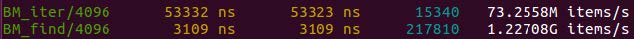
\includegraphics[width=0.9\textwidth]{content/3/chapter12/images/2.jpg}\\
圖12.2 - 使用迭代器和\texttt{find()}成員函數在索引數據存儲中進行搜索
\end{center}

退一步評估這個例子是非常重要的,它是軟件設計的經驗,而不是一個特定的優化技術。這個上下文中,\texttt{find()}成員函數是否比基於迭代器的搜索快得多並不重要。在設計階段,重要的是適當的實現可能會更快。它可能更快的原因是因為知道調用者的意圖。 

使用非成員和成員\texttt{find()}比較調用者提供的信息,當非成員\texttt{find()}函數調用容器接口時,我們告訴容器:“依次查看所有容器元素的值。”實際上並不需要這些操作,但這是給容器的信息,因為這是能通過迭代器接口傳遞的唯一信息。另一方面,成員\texttt{find()}允許發出以下請求:“以任意順序檢查所有元素,並告訴我是否至少有一個元素符合這個條件。”這個請求施加的限制要少得多,其將細節留給容器本身。在我們的示例中,實現者利用這種自由提供了更好的性能。

設計階段,可能不知道這樣的優化實現。成員\texttt{find()}的第一個實現也可以運行迭代器循環或調用\texttt{std::find\_if}。開發者也可能永遠不會優化這個函數,因為在應用程序中很少調用,並且不是性能瓶頸。但是軟件系統的壽命往往比預期的要長,而且重新設計是困難和耗時的。好的系統架構不應該限制系統的發展,甚至可以滿足添加新的特性和性能需求。

再次看到了性能友好型和性能敵對型設計之間的區別。當然,同樣的原則也適用於系統組件之間的交互,而不限於類。在設計響應請求或提供服務的組件時,允許請求者提供所有相關的信息,特別是表達請求背後的意圖。

由於幾個原因,這是一個更有爭議性的指南。首先,明顯地違背了類設計的主流方法:永遠不要為不需要特權訪問,且完全可以通過現有的公共API實現的任務實現(public)成員函數。關於這個問題,瞭解一下這樣做的幾個理由。首先,有人可能會說“可以以十倍的速度實現”並不真正符合“可以實現”的標準,因此該指導方針並不適用。相反,在設計階段甚至可能不知道需要這種性能。我們可能會違反的另一個重要規則是“不要過早地優化”,儘管不應該簡單地理解這條規則,這條規則的合理支持者經常會補充說,“但也不要過早地悲觀”。後者在設計的背景下,意味著做出設計決策,封閉未來的優化空間。

最大信息原則(或信息豐富的接口)的使用是一個平衡和合理判斷的問題。考慮到這一點,違反這條原則遠不如不遵守前面的規則那麼有害。若接口或約定暴露了不必要的信息,那麼很難從依賴它的客戶端收回這些信息。另一方面,如果接口不允許客戶端提供相關的意圖信息,那麼客戶端可能會執行低效率的實現。但在添加了信息更豐富的接口之後,一切就不同了,客戶端可以根據需要轉換到這個接口上。

因此,決定是否在一開始就提供一個信息豐富的接口,取決於以下幾個因素: 

\begin{itemize}
\item 
這個組件或組件之間的交互對性能至關重要的可能性有多大?雖然不鼓勵猜測特定代碼的性能,但需要知道有關組件的一般需求。每秒訪問數百萬次的數據庫很可能成為某個地方的性能瓶頸,而每月為員工提供兩次發薪地址的系統可以進行保守地設計,並在需要時再進行優化。

\item 
這個設計決策的影響有多大?若低效的實現氾濫,那當添加一個新的、更高級別的接口時,替換的難度有多大?一個類使用一到兩次,可以很容易地隨著它的客戶端更新。一個通信協議將成為整個系統的標準,並用於一個輕量級協議API中,該API將消息存儲在磁盤上長達數週或數月,從一開始就應該具有可擴展性,包括用於未來更豐富信息請求的選項。
\end{itemize}

通常情況下,這些選擇並不明確,取決於設計師的直覺和經驗。本書對前者有幫助,在實踐中可以解決後者的問題。 

在考慮不同設計決策的性能影響時,我們經常關注接口和數據組織。在下面的兩個部分中,我們將展開討論這兩個主題,從接口設計開始。








